\subsection{C1 -- Solar perihelion native window}\label{app:c1}
\paragraph{Native question.} Does the cited long-window orbital closure carry the predicted residual-duration support, dominant class $B^*$, torsional witness, and effective progress rate?
\paragraph{Native readout.}
\begin{itemize}
\item cited window $\omega_{\mathrm{sol,peri}}$
\item structural key \texttt{tetron:4:4:8}
\item frame count / $T_{\mathrm{eval}}=1200$ bip
\item weighting policy $w(\kappa)\equiv 1$
\item residual-duration chain
\end{itemize}
\paragraph{Native operator chain.}
\[
e_\alpha,\ e_\Omega,\ f
\;\to\;
b(\kappa)
\;\to\;
H_B
\;\to\;
B^*
\;\to\;
\Lambda_b
\;\to\;
A_B
\;\to\;
R_{\mathrm{rest}},\ v(\omega),\ T_{\mathrm{tors}}.
\]
\paragraph{Native output row.}
\begin{center}
\small
\begin{tabular}{lcccccc}
\toprule
Row & Key & $T_{\mathrm{eval}}$ [bip] & $B^*$ & $\Lambda_b$ & $R_{\mathrm{rest}}$ [trit/bip] & $T_{\mathrm{tors}}$ \\
\midrule
C1.A & tetron:4:4:8 & 1200 & 137 & 6 & $(1+8\ell_2)/24$ & 3 \\
\bottomrule
\end{tabular}
\end{center}
\paragraph{Temporal Conversion Block.} Temporal conversion is a normal chain-rule expansion on the cited native row. On this window, the perihelion witness is
\[
42.981975497467126\ \text{arcsec / century}.
\]
\paragraph{Native figure witness.}
\begin{center}
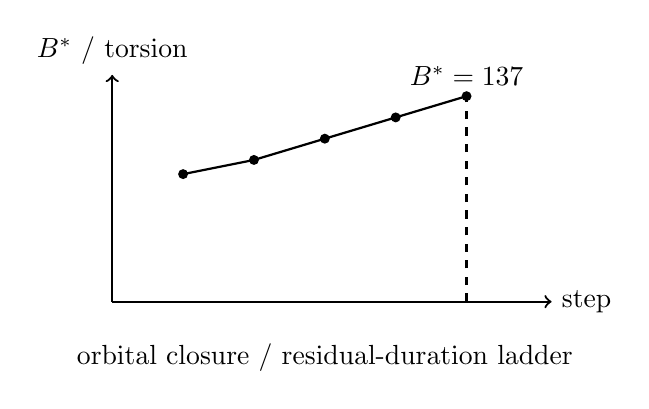
\begin{tikzpicture}[scale=0.9, thick]
\draw[->] (0,0) -- (6.2,0) node[right] {step};
\draw[->] (0,0) -- (0,3.2) node[above] {$B^*$ / torsion};
\foreach \x/\y in {1/1.8,2/2.0,3/2.3,4/2.6,5/2.9}{\fill (\x,\y) circle (2pt);} 
\draw (1,1.8)--(2,2.0)--(3,2.3)--(4,2.6)--(5,2.9);
\draw[dashed] (5,0)--(5,2.9);
\node[above] at (5,2.9) {$B^*=137$};
\node[below] at (3,-0.45) {orbital closure / residual-duration ladder};
\end{tikzpicture}
\end{center}
\paragraph{Hook / Evidence.} Use the cited orbital-closure and residual-support hooks from the main note.
